\graphicspath{{Figures/chapter3}}
\chapter{METHODOLOGY}
Initially, the proposed approach consist of determining the learning capability of proposed model for speed bump and pothole objects and then speed regulation of the vehicle prototype against the detected speed bump or pothole is followed.  The concept of the integrated system of Figure \ref{fig:units} consists of two units, namely, the detection unit and speed control unit. 
\begin{figure}[h]
    \centering
    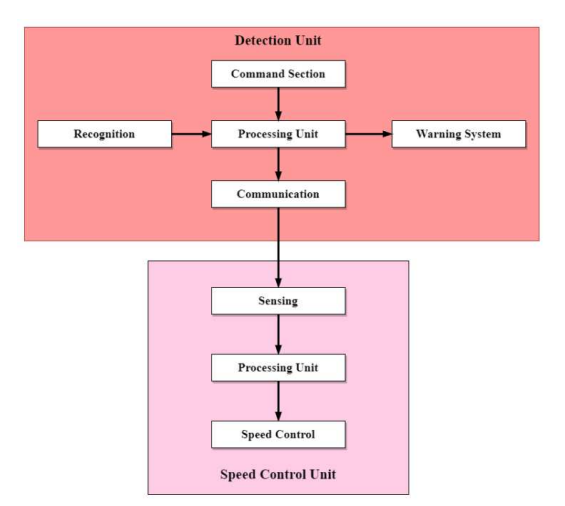
\includegraphics[scale=1]{Figures/chapter3/units.png}
    \caption{Diagram Representation of the System}
    \label{fig:units}
\end{figure}

\noindent
The detection unit deals with object recognition, communication with the speed control unit, warning instructions, and the command section to start, end or modify the system. Contrarily, the speed control unit deals with the sensing of the detection signal sent by the detection unit and controlling the vehicle speed accordingly.

\section{Vehicle Prototype Configuration}
The run-time implementation of the speed bump detection system requires an embedded vehicle prototype. For this purpose, we have chosen the Raspberry Pi 3B+ model(figure \ref{fig:hardware}(a)), which is equipped with a 1.4GHz 64-bit quad-core ARM Cortex-A53 CPU and 1GB LPDDR2 SDRAM module. These resources are sufficient for the operation of the proposed model. The Raspberry Pi 3B+ is also equipped with a monocular camera unit with an 8 megapixel resolution, which is capable of capturing static images of 3280 x 2464 pixels and supports 1080p30 video processing.

\noindent
In addition to the Raspberry Pi 3B+, we have also used a separate Arduino Uno microcontroller(figure \ref{fig:hardware}(b)) module for controlling the wheels and motors of the vehicle.
\begin{figure}[H]
    \centering
        \subfigure[]{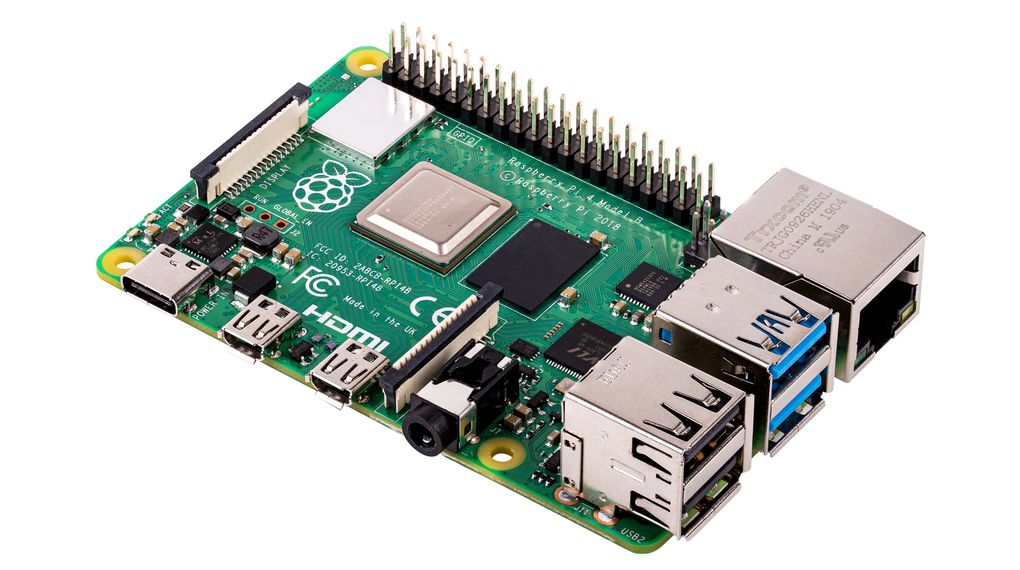
\includegraphics[width=0.45\textwidth]{Figures/chapter3/raspberrypi.jpg}}
        \subfigure[]{ 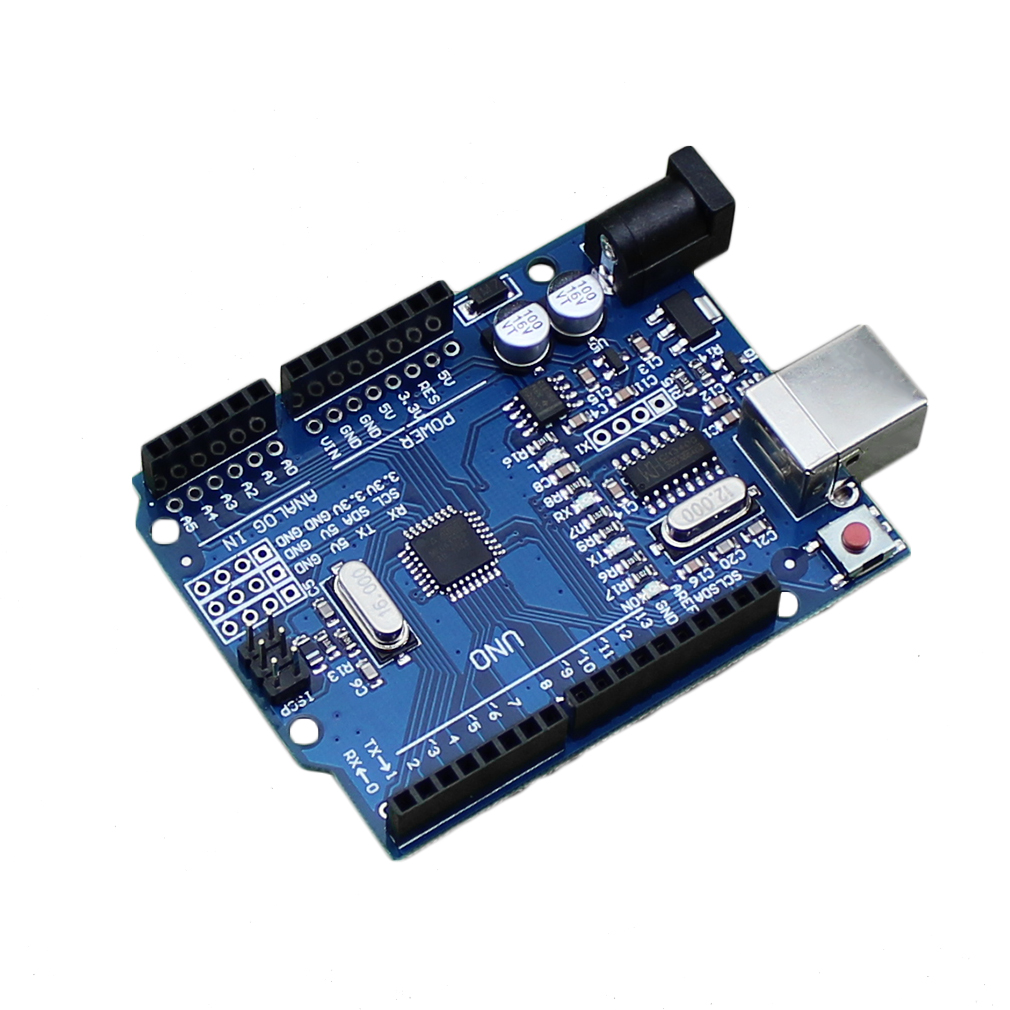
\includegraphics[width=0.45\textwidth]{Figures/chapter3/arduinouno.jpg}}
    \caption{Hardware Components}
    \label{fig:hardware}
\end{figure}

\noindent
\subsection{Hardware Components}
\subsubsection{Raspberry Pi}
The Raspberry Pi is a small, affordable, and versatile single-board computer that is popular among DIY enthusiasts and educators. It was developed in the United Kingdom by the Raspberry Pi Foundation with the goal of promoting the teaching of computer science in schools.

\noindent
One of the main advantages of the Raspberry Pi is its size and low power consumption, which makes it ideal for use in portable or embedded applications. It is also relatively cheap and easy to use, which makes it a popular choice for many projects, including self-driving cars. There are several ways that the Raspberry Pi can be used in a self-driving car project. For example, it can be used as the main computer for running the autonomous driving software, or it can be used to control various subsystems of the car, such as the motors, sensors, and cameras. 

\noindent
The Raspberry Pi is also capable of running a wide range of operating systems and programming languages, which makes it easy to integrate with other hardware and software components. This makes it a flexible platform for building and testing self-driving car prototypes.

\noindent
Overall, the Raspberry Pi is a powerful and cost-effective tool for developing self-driving car technology and other robotics applications. It is a great choice for those who are interested in learning more about autonomous vehicles and exploring the possibilities of this exciting field.
\subsubsection{Arduino UNO}
The Arduino Uno is a microcontroller board based on the ATmega328 microcontroller. It is one of the most popular boards in the Arduino family and is commonly used in a variety of DIY electronics projects, including self-driving cars.One of the main advantages of the Arduino Uno is its simplicity and ease of use. It has a user-friendly design, with a set of digital and analog input/output (I/O) pins that can be easily programmed using the Arduino Integrated Development Environment (IDE). This makes it a great choice for beginners who are just starting out with electronics and programming.

\noindent
In a self-driving car project, the Arduino Uno can be used to control various subsystems of the car, such as the motors, sensors, and cameras. It can also be used to interface with other hardware and software components, such as GPS modules and display screens. The Arduino Uno is also capable of running a wide range of programming languages and libraries, which makes it easy to integrate with other technologies and build complex systems. It is a versatile and powerful platform for developing self-driving car technology and other robotics applications.
\begin{table}[H]
\centering
\begin{tabular}{|l|l|}
\hline
\textbf{Module} & \textbf{Specification}       \\ \hline
Camera          & 8 megapixels, 1080p30,780p60 \\ \hline
DC-motor        & 5v, 20mA, 2000RPM            \\ \hline
Buzzer          & 5v, 20mA                     \\ \hline
H-Bridge        & 5v, 35mA                     \\ \hline
\end{tabular}
\caption{Specification Of Hardware Modules}
\label{tab:hardwarecomp}
\end{table}
\subsection{Serial Communication}
Serial communication is a method of transmitting data serially, or one bit at a time, over a communication channel or computer bus. It is often utilized for transferring data between devices, such as microcontrollers and computers. The Raspberry Pi and Arduino are two popular microcontroller boards that are equipped with serial communication interfaces, allowing for a serial connection to be established between them. To establish a serial connection between the Raspberry Pi and Arduino, a serial cable or wireless serial module must be used to connect the two boards. Additionally, the serial port settings on both boards must be properly configured, including the baud rate and parity. Once the connection is established, serial libraries or terminal programs can be utilized to send and receive data between the boards.

\noindent
Serial communication is a simple and reliable method for exchanging data between the Raspberry Pi and Arduino, and it is frequently employed in various projects, including self-driving cars, robotics, and Internet of Things (IoT) applications. The Raspberry Pi sends a message to the Arduino through the serial port (UART) to request a certain action, such as turning on an LED. The Arduino receives the message and performs the requested action. This process allows for the integration of the Raspberry Pi and the Arduino, allowing for the combination of the Raspberry Pi's advanced computing capabilities with the Arduino's ability to control electronic devices.

\noindent
The Raspberry Pi and Arduino modules are connected using serial communication, allowing the Raspberry Pi to capture frames and identify speed bump objects within bounding boxes. The Raspberry Pi also calculates the distance between the vehicle and the object and sends the processed information to the Arduino, which then modifies the driving behavior of the vehicle accordingly. The developed prototype vehicle can be seen in Figure \ref{fig:carconfig}. 

\noindent
It is equipped with the necessary hardware components, including the Raspberry Pi 3B+ and Arduino Uno, as well as a camera unit and motors for controlling the movement of the vehicle. The prototype is capable of detecting speed bumps and potholes in real-time and adjusting its speed and trajectory accordingly, making it a valuable asset for the safe and efficient operation of autonomous vehicles.
\begin{figure}[H]
    \centering
    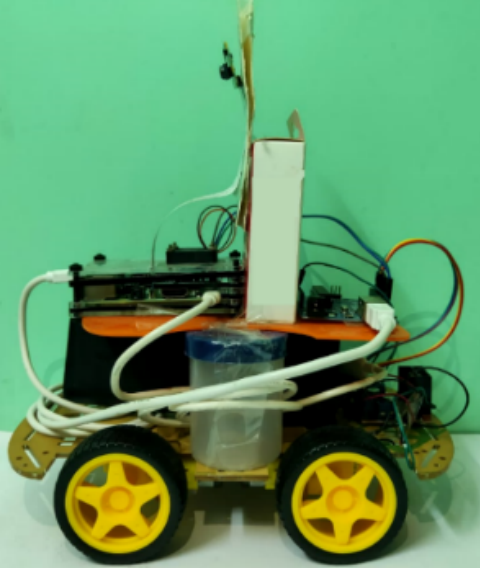
\includegraphics[scale=1]{Figures/chapter3/carconfig.png}
    \caption{Prototype Vehicle}
    \label{fig:carconfig}
\end{figure}


\section{Speed Bump and Pothole Detection}
This section presents an overview of the methods and techniques used in the development of the application for detecting and navigating speed bumps and potholes with autonomous vehicles. The focus of this section is on providing a comprehensive understanding of the steps and techniques involved in the development process.
\noindent
We begin by discussing the creation of the dataset, which is a critical step in any machine learning project. The dataset is used to train and test the network, and it is important that it accurately represents the real-world scenarios in which the system will be used. We also describe the preprocessing techniques applied to the dataset in order to prepare it for use in the network.

\noindent
Next, we describe the training and testing of the network for both classification and detection tasks. Classification involves identifying the type of road hazard (e.g., speed bump or pothole), while detection involves locating and measuring the size and position of the hazard in the road. We describe the specific methods and techniques used to train and test the network for these tasks.

\noindent
Overall, this section aims to provide a thorough understanding of the methods and techniques used in the development of the application for detecting and navigating speed bumps and potholes with autonomous vehicles.
\subsection{Training Data Generation}
The following steps are involved in dataset generation:
\begin{figure}[h]
    \centering
    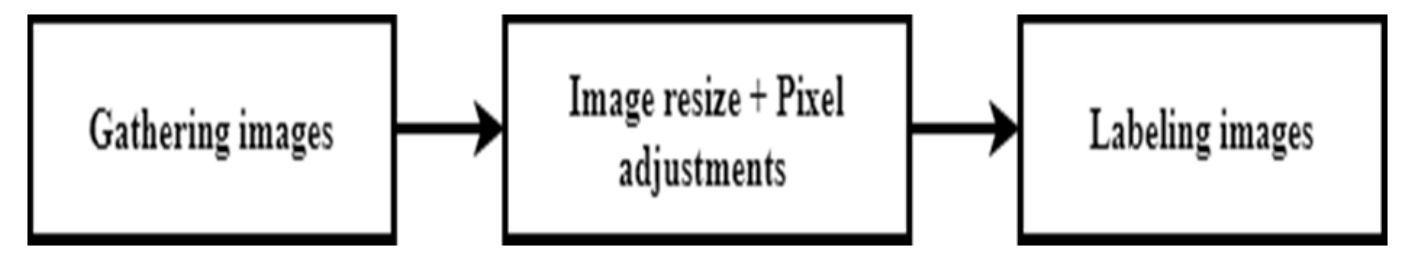
\includegraphics[scale=0.5]{Figures/chapter3/dataset_steps.png}
    \caption{The steps involved in generating training data}
    \label{fig:dataset_steps}
\end{figure}

\noindent
For this Seminar the sample images used in this study were collected from different roads in Rajshahi and Tangail, Bangladesh, totaling approximately 3000 images. Of these, 2500 images were selected for use in training the model, comprising 1000 images of potholes, 900 images of marked speed bumps, and 600 images of unmarked speed bumps. These images were chosen to provide a representative sample of the various road hazards that the model would be expected to encounter in real-world scenarios.

\noindent
The image resolution was carefully considered in the selection process, as the size of the images can have a significant impact on the training time of the model. After evaluating various options, it was determined that a resolution of 800*600 pixels was optimal for this application. This size provided a good balance between image quality and training efficiency.

\noindent
Pixel resizing was also an important consideration in the process of preparing the images for training. If the images are too large, the training time for the model can become prohibitively long. On the other hand, if the images are too small, important details may be lost, which can negatively impact the performance of the model. In this study, the images were resized to a maximum of 200 KB in order to minimize training time without sacrificing image quality.

\noindent
Finally, the software LabelImg was used to construct Extensible Markup Language (XML) files for each image, which contained the necessary annotation data for training the model. These XML files specified the location and dimensions of the road hazards in each image, allowing the model to learn to detect and classify them accurately

\subsection{Training Model}
This study employs the SSD MobileNet v2 Quantized COCO model to develop a learned system for detecting and navigating speed bumps and potholes with autonomous vehicles. The MobileNet model is based on depthwise separable convolutions, which are a type of factorized convolutions that decompose a standard convolution into a depthwise convolution and a 1x1 convolution called a pointwise convolution. This architecture has been designed to be computationally efficient and well-suited for use in resource-constrained environments such as embedded systems.
\subsubsection{Single Shot Multibox Detector}
\noindent
The SSD (Single Shot Multibox Detector) method is a popular approach for object detection tasks, and it uses a feed-forward convolutional network to generate a fixed-size collection of bounding boxes and scores for the presence of object class instances in those boxes. The SSD method uses a CNN architecture that consists of a series of convolutional and max-pooling layers, followed by a series of fully-connected (fc) layers. The convolutional layers are used to extract features from the input image, while the max-pooling layers are used to down-sample the feature maps and reduce the number of parameters in the network. SSD’s architecture(as shown in Figue \ref{fig:ssd_img}) builds on the venerable VGG-16 architecture, but discards the fully connected layers. 
\begin{figure}[h]
    \centering
    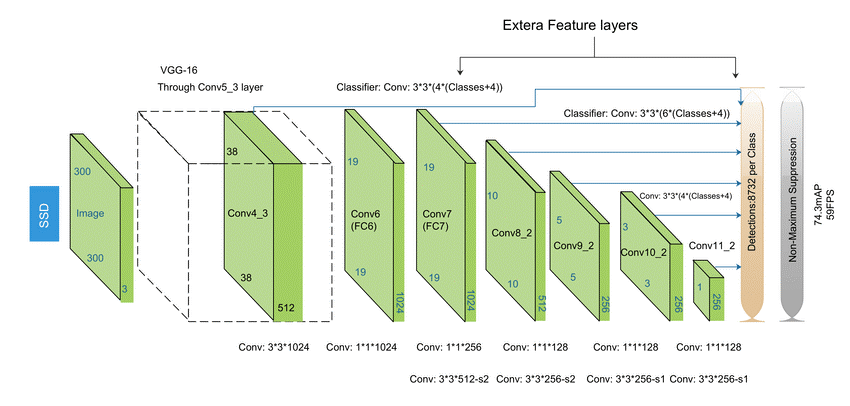
\includegraphics[scale=0.7]{Figures/chapter3/ssd_architecture.png}
    \caption{Single Shot Multibox Detector Architecture}
    \label{fig:ssd_img}
\end{figure}

\noindent
The fc layers are used to make the final predictions for the bounding boxes and class scores. One of the key features of the SSD method is the use of anchor boxes, which are fixed-size bounding boxes that are used as reference points for predicting the locations of object instances in the image. The anchor boxes are defined at multiple scales and aspect ratios, and they are used to predict the locations of object instances at different scales and in different parts of the image.


\noindent
The SSD method also uses a technique called multibox, which involves using multiple sets of fc layers to predict the bounding boxes and class scores for the object instances. Each set of fc layers is responsible for predicting the bounding boxes and class scores for a particular scale and aspect ratio of anchor boxes. This allows the network to make predictions for object instances at different scales and in different parts of the image.This method is known for its efficiency and ability to handle a large number of classes, making it well-suited for applications such as autonomous vehicle obstacle detection.
\subsubsection{MS COCO Dataset}
\noindent
The MS COCO (Microsoft Common Objects in Context) dataset is a large-scale dataset for image segmentation, object detection, keypoint identification, and captioning. It was developed by Microsoft Research and contains 328K images, making it one of the largest and most comprehensive datasets of its kind. The images in the MS COCO dataset are drawn from a wide range of sources, including the Internet and professional image libraries, and they cover a wide variety of object categories and scene types. The dataset is designed to be representative of the types of images that are commonly encountered in real-world applications, and it is widely used as a benchmark for evaluating the performance of object detection and image segmentation algorithms. One of the key features of the MS COCO dataset is the extensive annotation provided for each image. Each image is annotated with a set of bounding boxes that define the location and dimensions of the objects in the image, as well as a set of labels that identify the class of each object. In addition, the dataset also includes annotations for keypoints, which are points of interest on the objects in the image, and captions, which provide a natural language description of the content of the image. 

\begin{figure}[h]
    \centering
    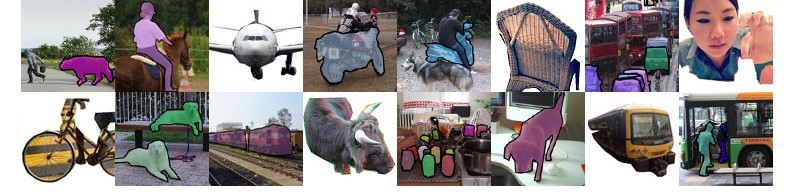
\includegraphics[scale=0.6]{Figures/chapter3/coco-examples.jpg}
    \caption{MS-COCO Dataset Examples}
    \label{fig:coco_eg}
\end{figure}

\noindent
We have chosen the SSD MobileNet v2 Quantized COCO model for this application due to its ability to provide good performance on a Raspberry Pi 4B while still being computationally efficient. The quantized version of the model has been designed to offer minimal model size and fastest performance at the expense of some accuracy compared to the full-precision version of the model.

\noindent
Overall, the combination of the SSD method and the MobileNet v2 Quantized COCO model represents a practical and effective solution for detecting and navigating road hazards in real-time with autonomous vehicles. The combination of efficiency, good performance, and low computational requirements make this model well-suited for use in resource-constrained environments such as autonomous vehicle platforms.

\noindent
SSD implements several enhancements, including multiscale features and default boxes, to make up for the reduction 
in accuracy. The SSD object detection composes of 2 parts: 
\begin{itemize}
    \item Extract feature maps and
    \item Convolutional predictors to detect objects.
\end{itemize}
 VGG16 is used by SSD to extract feature maps.The reason VGG-16 was used as the base network is because of its strong performance in high quality image classification tasks and its popularity for problems where transfer learning helps in improving results. Instead of the original VGG fully connected layers, a set of auxiliary convolutional layers (from conv6 onwards) were added, thus enabling to extract features at multiple scales and progressively decrease the size of the input to each subsequent layer.The architecture of VGG-16 is illustrated in Figure \ref{fig:vgg16}.
 \begin{figure}[h]
     \centering
     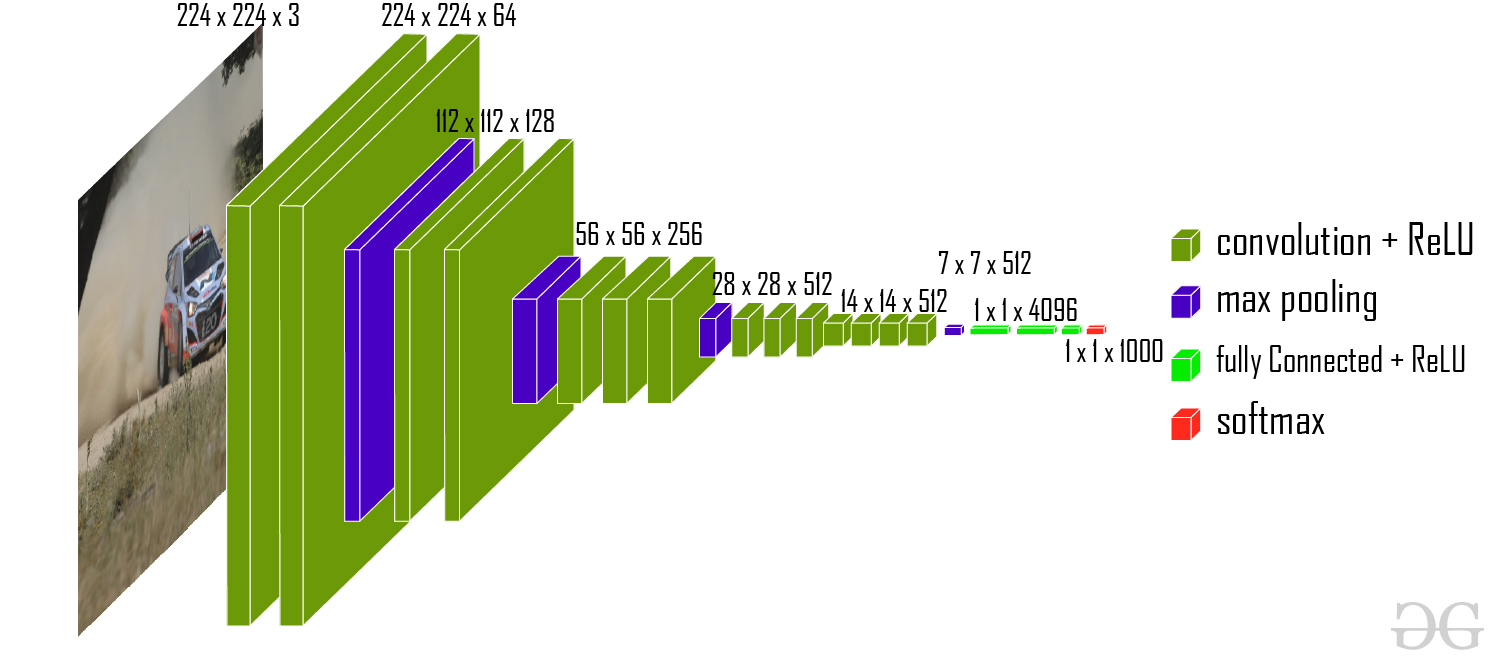
\includegraphics[scale=0.3]{Figures/chapter3/vgg16.jpg}
     \caption{VGG-16 Architecture}
     \label{fig:vgg16}
 \end{figure}

 \noindent
The Conv4\_3 layer is then used to detect objects. SSD calculates both the class scores and the location using small convolution filters. After retrieving the feature maps, SSD uses 3 x 3 convolution filters on each cell for making predictions. Each filter produces 25 channels, with 21 scores for each class and one boundary box for each. For identifying larger-scale objects, SSD employs lower resolution layers. The 4×4 feature maps, for example, are utilized for larger scale objects. Each feature map layer has a scale value defined by SSD. Conv4\_3 detects objects at the smallest size of 0.2 (or 0.1 in some cases) on the left, then grows linearly to the rightmost layer at a scale of 0.9 on the right.

\noindent
Then the width and the height of the default boxes are 
calculated as: 

\begin{flalign}
     w &= scale\sqrt{aspect\ ratio} &\\
    h &= \frac{scale}{\sqrt{aspect\ ratio}} &\\
    SSD\ adds\ an\ extra\ default\ box\ with\ scale: \nonumber &\\
    scale &= \sqrt{scale.aspect\ at\ next\ level} &
\end{flalign}

\noindent
The SSD (Single Shot Multibox Detector) method makes predictions of two types: positive and negative matches. When evaluating the cost of localization (the mismatch between the predicted bounding box and the ground truth bounding box), SSD only considers positive matches. A positive match is defined as a prediction with an intersection over union (IoU) greater than 0.5 between the ground truth bounding box and the associated default bounding box. Conversely, a prediction with an IoU less than 0.5 is considered a negative match. This matching strategy encourages the prediction of shapes that are more closely aligned with the corresponding default bounding box.
\begin{figure}[H]
    \centering
        \subfigure[]{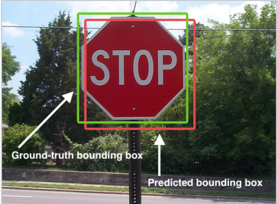
\includegraphics[width=0.45\textwidth]{Figures/chapter3/iou1.png}}
        \subfigure[]{ 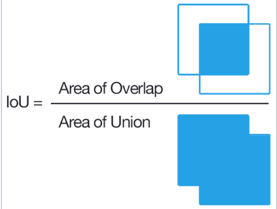
\includegraphics[width=0.45\textwidth]{Figures/chapter3/iou2.png}}
    \caption{IoU Calculation}
    \label{fig:iou_main}
\end{figure}
\begin{figure}[H]
    \centering
    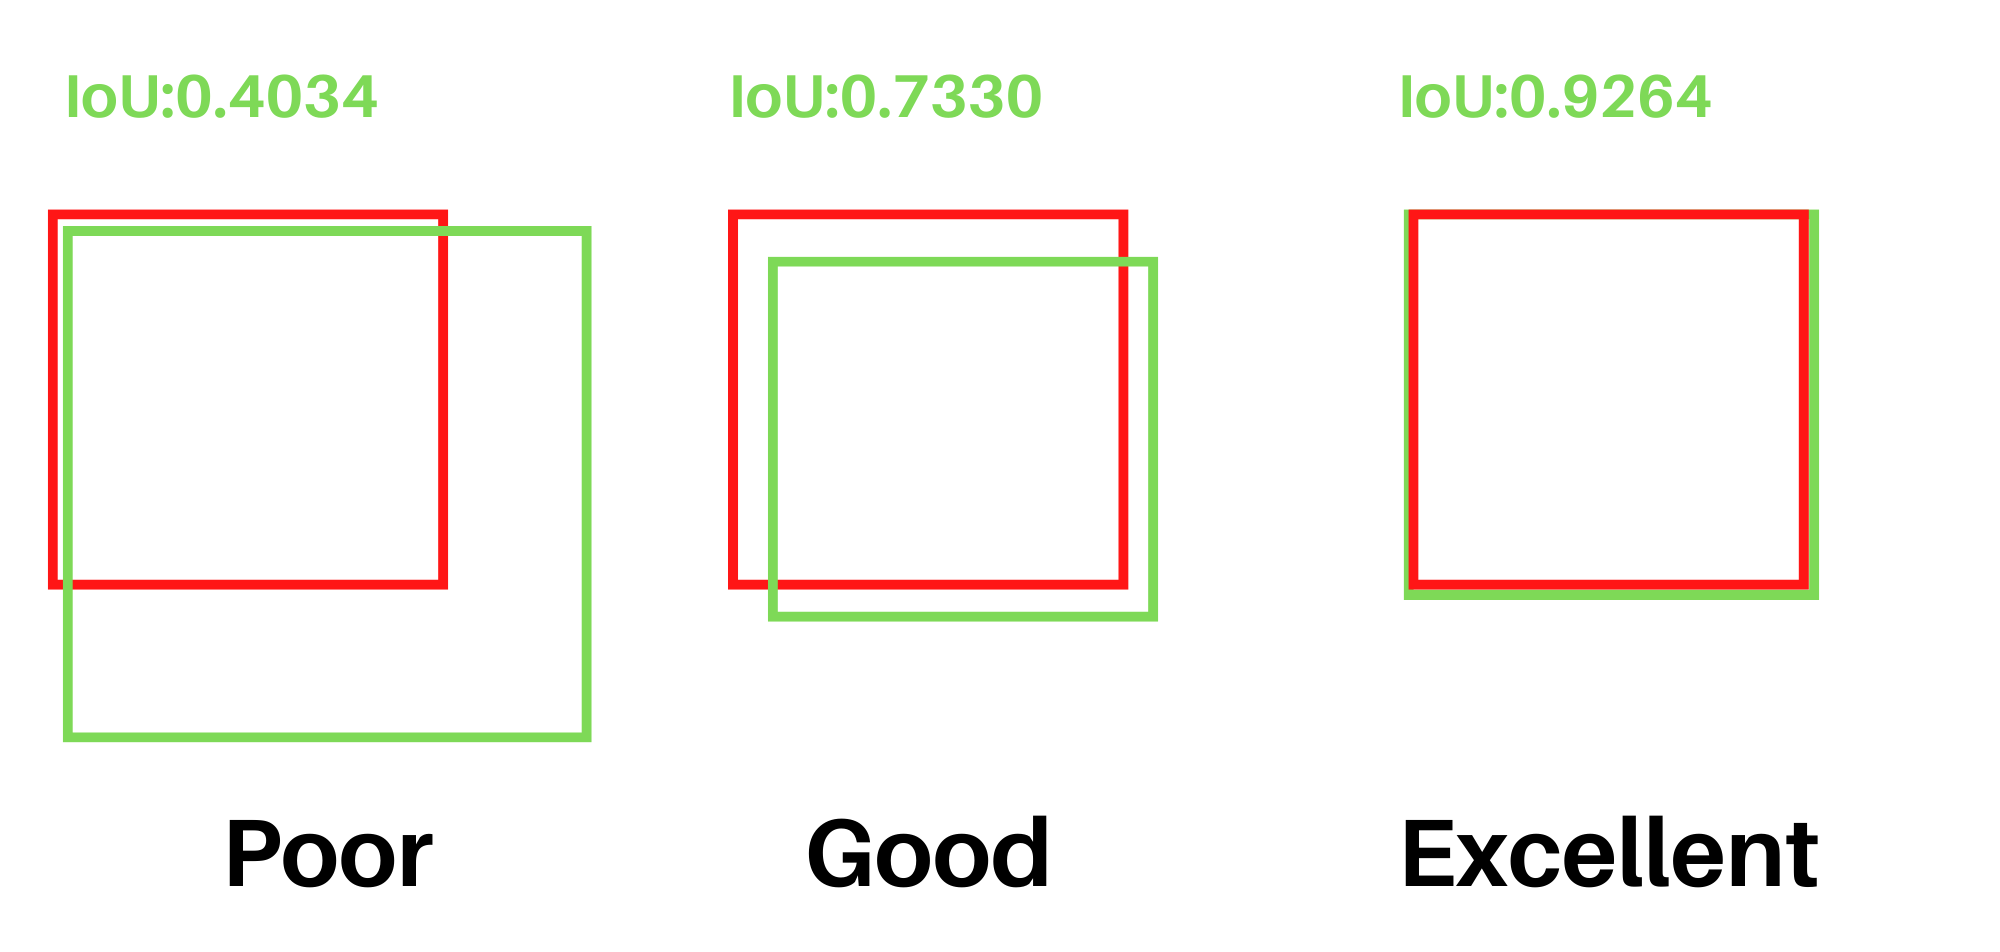
\includegraphics[scale=0.8]{Figures/chapter3/iou3.png}
    \caption{IoU Threshold Ranking}
    \label{fig:iou3}
\end{figure}
\subsection{Loss Function}
The mismatch between the predicted boundary box and the ground truth box is known as the localization loss. It is typically calculated using a measure such as the intersection over union (IoU) between the predicted and ground truth bounding boxes.This matching strategy is used to encourage predictions that are more closely aligned with the corresponding default boxes and to reduce the impact of negative matches on the overall localization loss.By minimizing the localization loss, the SSD method aims to improve the accuracy and precision of the object detection model in predicting the locations and sizes of objects in an image. The localization loss between the predicted box \textit{l} and the ground truth box \textit{g} is defined as the smooth L1 loss with \textit{cx,cy} as the offset to the default bounding box \textit{d} of width \textit{w} and height \textit{h}\cite{R4}.
\begin{flalign}
    l_{loc} &=\sum_{i\in Pos\ m\in\{cx,cy,w,h\}}^{N}\sum\hat{x}_{ij}^ksmooth_{L1}(l_i^m-\hat{g}_j^{m})\nonumber\\
    \hat{g}_j^{cx} &= \frac{ \hat{g}_j^{cx}- \hat{d}_i^{cx}}{ \hat{g}_i^{w}}\\
     \hat{g}_j^{cy} &= \frac{ \hat{g}_j^{cy}- \hat{d}_i^{cy}}{ \hat{d}_i^{h}}\\
      \hat{g}_j^{w} &= \log\log(\frac{ \hat{g}_j^{w}}{ \hat{d}_i^{w}})    \\
      \hat{g}_j^{h} &= \log\log(\frac{ \hat{g}_j^{h}}{ \hat{d}_i^{h}}) \\
        x_{i\ j}^{p} &= \begin{cases}
            1,& \text{if IoU>0.5 between default box i and ground true box j on class p}\\
    0,              & \text{otherwise}   
         \end{cases}        
\end{flalign}
\subsection{Model Implementation}
In order to deploy the trained model on a low-power edge device such as the Raspberry Pi, it is necessary to convert it to a format that is compatible with the TensorFlow Lite framework. TensorFlow Lite is a lightweight version of the TensorFlow framework that is specifically designed for deployment on mobile and embedded devices. Once the trained model has been converted to a TensorFlow Lite file, it can be transferred to the target device and executed using the TensorFlow Lite runtime.
\noindent
In this case, the trained model was converted to a TensorFlow Lite file and transferred to a Raspberry Pi device. The Raspberry Pi is a low-cost, low-power single-board computer that is widely used in a variety of embedded and IoT (Internet of Things) applications. By using the Raspberry Pi camera as the input sensor, the converted model was able to detect the desired object in real-time on the edge device. This allows the model to be deployed in a variety of settings where low-power, low-cost, and real-time performance are key requirements.
\subsection{Object to camera distance calculation}
Once the object is detected that is enclosed in a bounding
box, the very next approach for an IVS is to measure the
distance of this object in real world. Calculating this distance is necessary aspect of IVS; as it has to change its driving behavior according to the detected speed bump. Work in
[41] and [42] involves distance measurement for detected
vehicle object in road environment. The performance under
standard condition was steady but requires high computation.
To overcome this, simple logic is employed to determine the
actual distance of object to the camera. It is obvious that
whenever an object moves away from the camera its size is
reduced and increased when it moves closer to the object.
Using this general perception, the bounding box that holds
speed bump object assist to determine the distance from the
camera and can be visualized in figure \ref{fig:dist_calc}.
\begin{figure}[H]
    \centering
    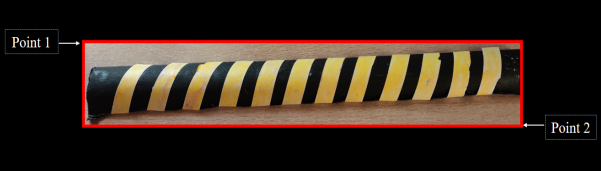
\includegraphics[]{Figures/chapter3/dist_calc.png}
    \caption{Real time detection result}
    \label{fig:dist_calc}
\end{figure}

\noindent
The left and right boundary markings are considered as Point 1 and Point 2. The difference of Point 2 and Point 1 is easily obtainable and measured in pixels. The difference between these two points varies with the scale of object and depends on the vehicle movement towards the speed bump object. It allows to derive the linear equation for calculated difference between Point 2, Point 1 and the tentative distance D1 and D2. For example, the D1 for a random position on track of speed bump to the vehicle position is taken as 60 cm, and let the difference between Point 2 and Point 1 is 70 pixels. Similarly, another distance D2 is set to 90 cm for speed bump to the vehicles fix position and pixel difference between similar points is 45 pixels. Using these parameters we solve equations of y=mx+c for 60=70m+c and 90=45m+c. 

\noindent
Once the parameters of equation is determined, then the
value of m and c will be utilized to calculate the distance
between object and vehicle on every movement (in centimeter)
towards the speed bump. The moment when vehicle comes
closer to object, its size gets increased and is computed with
dynamic change in pixel positions (Point 2 and Point 1). This
helps to represent the actual distance which is closely related to the focal length of camera in real time scenario.

\section{Algorithm And Flowchat}
In the context of this seminar topic, the algorithm is used to detect and classify speed bumps and potholes in the road ahead of an autonomous vehicle. The algorithm begins by collecting input images from the front-facing camera of the raspberry pi as it drives along the road. The input images are then processed by a Single Shot Multibox Detector (SSD) trained to detect and classify speed bumps and potholes. The SSD generates a set of bounding boxes and scores for the detected objects, which are then passed through a non-maximum suppression step to generate the final set of detections. Based on the location and size of the detected speed bumps and potholes, the algorithm calculates the appropriate speed and trajectory to safely navigate the obstacles. It also includes mechanisms to handle false positives and false negatives, as well as to update and refine the model based on new data.The algorithm is designed to enable the autonomous vehicle to detect and safely navigate speed bumps and potholes in real-time, improving the safety and efficiency. The general algorithm for the project is given below: 

\noindent
Step 1: Power supply to the components. \\
Step 2: The python script for detection is initialized on the Raspberry Pi \\
Step 3: Script checks the video feed for speedbump or pothole \\
Step 4: If detected, it blinks the LED, turns on the buzzer, and sends the signal to Arduino.\\ 
Step 5: Arduino slows down the motors to a predetermined value. \\
Step 6: Arduino checks if the detection signal still 
available or not. \\
Step 7: If available, it maintains the reduced speed. \\
Step 8: Else it speeds up to the initial speed. \\
Step 9: Raspberry Pi turns off the LED \& Buzzer. \\
Step 10: Step 3 to step 9 is repeated until the device is turned off. \\
Step 11: Cut the power supply to end the process.

\noindent
To illustrate a procedure or a program, a flowchart is the graphical or pictorial representation of an algorithm using numerous symbols, shapes, and arrows. The flowchart-based on the algorithm of the proposed system is given below: 
\begin{figure}[h]
    \centering
    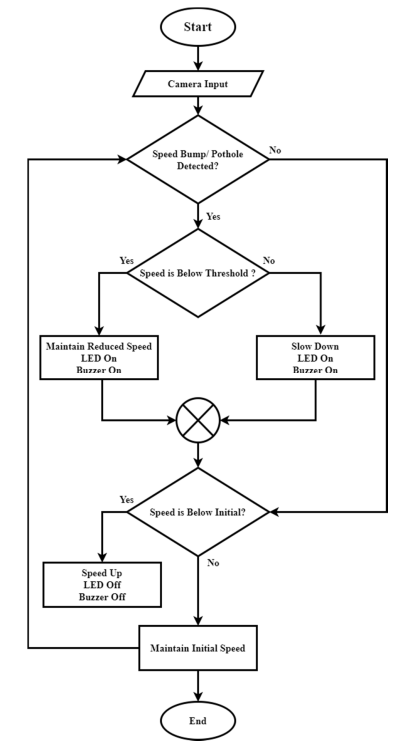
\includegraphics[scale=1]{Figures/chapter3/flowchart.png}
    \caption{Flow Chart of Proposed System}
    \label{fig:flowchart}
\end{figure}